\documentclass[annual]{acmsiggraph}
\usepackage{relsize} 

\usepackage{amsmath} 

\usepackage{algorithm} 

\usepackage[noend]{algorithmic}

\usepackage{listings}

\lstset{language=HTML}

\TOGonlineid{163}

\TOGvolume{} 

\TOGnumber{} 

\TOGarticleDOI{} 

\TOGprojectURL{} 

\TOGvideoURL{} 

\TOGdataURL{} 

\TOGcodeURL{}

\newcommand{\Acronym}[1]{\ensuremath{{\small{\texttt{#1}}}}}
\newcommand{\Name}{\Acronym{Camgaze.js}} \newcommand{\False}{\Constant{false}}
\newcommand{\True}{\Constant{true}}
\newcommand{\Symbol}[1]{\ensuremath{\mathcal{#1}}}
\newcommand{\Function}[1]{\ensuremath{{\small \textsc{#1}}}}
\newcommand{\Constant}[1]{\ensuremath{\small{\texttt{#1}}}}
\newcommand{\Var}[1]{\ensuremath{{\small{\textsl{#1}}}}}
\newcommand{\argmin}[1]{\underset{#1}{\operatorname{arg}\,\operatorname{min}}\;}

\title{Camgaze.js: Browser-based Eye Tracking and Gaze Prediction using
JavaScript}

\author{Alexander Wallar \thanks{email: aw204@st-andrews.ac.uk} \\ Aleksejs
Sazonovs \thanks{email: as245@st-andrews.ac.uk} \\ University of St Andrews
\and Christian Poellabauer \thanks{email: cpoellab@nd.edu} \\ Patrick Flynn
\thanks{email: flynn@nd.edu} \\ University of Notre Dame}

\pdfauthor{Alexander Wallar, Christian Poellabauer, Patrick Flynn, Aleksejs
Sazonovs}

\keywords{gaze prediction, eye detection, pupil detection, low-cost eye
tracking, linear calibration, JavaScript eye tracker, in-browser eye tracking}

\date{\today}

\begin{document}

\maketitle

\begin{abstract}

Eye tracking is a difficult problem that is usually solved using specialised
hardware and therefore has limited availability due to cost and deployment
difficulties. We describe $\Name$, a client-side Javascript library that is
able to estimate the point of gaze using only commodity optical cameras without
relying on any external application installed besides a web-browser. We conduct
experiments using $\Name$ to show the usability of such a system.  We also
discuss the challenges and applications of using an in-browser eye tracking
system. Since the described eye tracker works inside the browser without any
additional installation setup, it provides a solution to a larger deployment of
eye tracking systems.

\end{abstract}

\begin{CRcatlist}\CRcat{I.4.8}{Image Processing and Computer Vision}{Scene
Analysis}{Tracking} \CRcat{I.4.9}{Image Processing and Computer
Vision}{Applications}{};

\end{CRcatlist}

\keywordlist

%\TOGlinkslist

\copyrightspace

\section{Introduction}

Eye tracking is a challenging problem that has been a topic of research
since the 19th century \cite{Wade2010}. Currently, it is mostly viewed as a
problem in Computer Vision. The majority of eye tracking solutions available on
the market today are a combination of software and specialised hardware.
Hardware based solutions employ a variety of technologies such as head-mounted
cameras and magnetically actuated lenses. State of the art solutions can allow
predicting the gaze point with high precision.  Despite that, carrying out eye
tracking experiments remains an issue –- it is expensive, requires complicated
deployment and calibration and, in most cases, has to be carried out in a
controlled environment.

In recent years, it has been shown \cite{SanAgustin2009}\cite{Sewell2010}
that it is possible to use commodity cameras, often built into modern
computers to perform eye tracking with promising quality. Deployment of such
systems is relatively simple, but in the described cases it is tied to specific
computer platforms \cite{holland2012eye}.

Web applications are “rich” websites that are able to run without external
plugins inside the browser. Recently, web browsers have evolved to adapt to
the market’s requirements -- new technologies have risen, allowing web
application to be increasingly interactive. For example, WebRTC (Web Real-Time
Communication) is an API that aims to enable in-browser audio and video
communication. As of September 2013, WebRTC is supported in the stable versions
of Google Chrome and Mozilla Firefox. A recent report
\cite{DisruptiveAnalysis2013}, claims that by 2016 there will be
3 billion capable devices and 1 billion individual users of WebRTC-enabled
devices.

In this paper, we describe $\Name$ -- a Javascript library that uses WebRTC to
obtain the video from built-in or USB cameras and measures the point of gaze.
It has the potential to be deployed in a wide range of applications such as
entertainment, healthcare and user-interface design



\section{Challenges}

The deployment of eye tracking systems on a wide range of hardware creates
number of challenges challenges.  The cameras that are built-in (or supplied
with) consumer devices vary greatly: there is no standard resolution, color
profile, brightness level, or physical position. Currently, WebRTC provides
very limited options for changing any of the parameters of the camera that is
providing a stream. This problem can be partially addressed by defining
individual profiles for a variety of popular devices. The identification of the
device is not a trivial task by itself, but services like DeviceAtlas
\cite{DeviceAtlas2013} solve it by looking at a variety of factors, such as
browser’s User-Agent and screen resolution.  Unfortunately, this approach would
be mostly applicable for handheld devices and not commodity PCs.

The client-side Javascript environment in which $\Name$ runs sets some
constraints. There are no comprehensive computer vision libraries available in
JavaScript as of this writing.  There is also currently no “simple” way to port
native C/C++ code, which are languages in which popular libraries such as
OpenCV are written in.  Projects like Emscripten are making early attempts to
allow translation of LLVM bitcode code to Javascript, potentially allowing to
port some of the well-established computer vision libraries to Javascript in
the future. For now, we had to create a custom implementation of connected
component detection and image moment calculation to use in $\Name$.

Despite some of the described difficulties, we believe that a combination of
Javascript and WebRTC is a reasonable technological stack on which a scalable
eye tracking solution can be built.

\section{Implementation}

\textbf{Algorithm 1} shows a high-level overview of $\Name$. The algorithm
first executes a calibration phase. Once the system is calibrated, it is able
to project the gaze position of the user. 

\begin{algorithm}
\caption{Pseudocode for $\Name$}
\label{algo:Main}
\begin{algorithmic}[1]
\setcounter{ALC@line}{0}

\vspace*{1mm}

\STATE $\Symbol{F} \leftarrow \Function{InitGazeMapping}()$

\WHILE{$\Function{StillCalibrating()} == \True$}
\STATE $P_{list} \leftarrow \Function{DetectPupils()}$
\STATE $\Symbol{G} \leftarrow \Function{DetermineGazeMetric}(P_{list})$
\STATE $\Symbol{F} \leftarrow \Function{Calibrate}(\Symbol{G}, \Symbol{F})$
\ENDWHILE

\WHILE{$\Function{SessionFinished()} == \False$}
\STATE $P_{list} \leftarrow \Function{DetectPupils()}$
\STATE $\Symbol{G} \leftarrow \Function{DetermineGazeMetric}(P_{list})$
\STATE $\Function{ProjectGazeOntoScreen}(\Symbol{F}(\Symbol{G}))$
\ENDWHILE

\end{algorithmic} 
\end{algorithm}

$\Name$ executes three steps in order to predict the position on the screen
that the user is looking at. Firstly, the pupils are detected. Then the
positions of these pupils with reference to the eye are used to determine a
\emph{gaze metric}. This gaze metric is then calibrated and mapped to a
position on the screen.

\subsection{Pupil Detection}

Detecting the pupils enables $\Name$ to determine the gaze direction. Firstly,
the frame is converted to grayscale and the eye is detected using the
Viola-Jones object detection framework \cite{Viola01}.  The region of interest
(ROI) is then thresholded for an array of different grayscale shades in order
to produce binary images.  Connected components are then detected on these
binary images.  All of the detected connected components are stored as possible
pupils.  Out of these possible pupils, the one with the minimum overall error
is designated as the pupil.  Below are the expressions to be minimized.
\begin{eqnarray} \Function{err}_{\alpha}(p) &=& \frac{ \mathlarger{\sum}_{c \in
Corners}{ \vert \frac{\pi}{4} - \Function{arctan}( \vert \frac{p_y - c_y}{p_x -
c_x} \vert) \vert } }{\pi} \\ \Function{err}_{size}(p) &=& \frac{ \vert
\Var{avgPupilSize} - \Function{size}(p) \vert }{2} \end{eqnarray}

In these equations, $p$ represents a possible pupil and thus has an $(x, y)$
position and a size. The $Corners$ set refers to the corners of the Haar
bounding rectangle surrounding the eye. $\Function{err}_{\alpha}$ s an angular
distance between the centroid of the connected component and the center of the
Haar bounding rectangle.  We use angle deviation instead of pixel distance for
this metric because we assume that the pupil would not always reside
immediately in the center of the boundary rectangle. A direct pixel distance
might yield different, and perhaps more suitable, connected components.  The
angle deviation acts a weak error function in order to be more lenient without
the use of constants.  Once the connected component with the minimum error is
extracted, its center is returned.

$\Function{err}_{size}$ is the difference between the scaled area of the
detected blob and the average scaled area of a general pupil. This means that
during the thresholding process, out of the  array of connected components
detected with minimal $\Function{err}_{\alpha}$, the one that has the area
closest to that of an average pupil will be returned.

Using a combination of these two error functions, we are able to detect the
pupils accurately and derive a gaze metric.

\begin{figure}[ht]

    \centering

    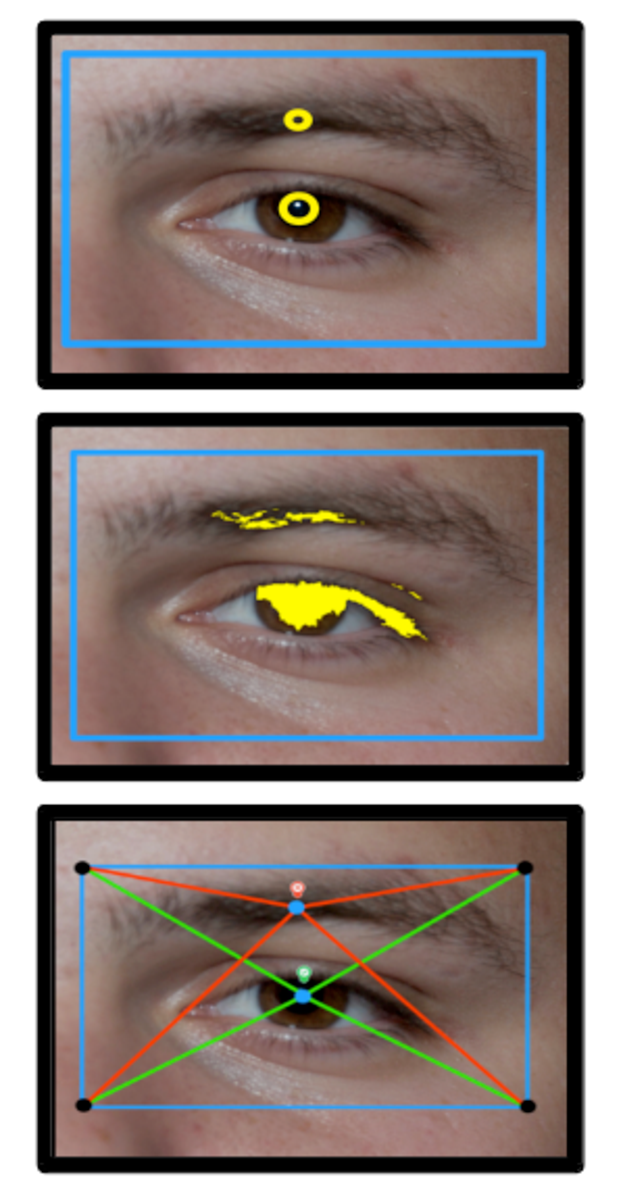
\includegraphics[width=1.5in]{figs/pupilDetection.pdf}

    \caption{Pupil Detection Process}

\end{figure}

\textbf{Figure 1} depicts the process of pupil detection. The first photoshows
the connected component segmentation. In the second image, the centers of the
connected components are extracted. The final image shows the deviation of the
$\Function{err}_{\alpha}$ for the two connected components.  Since the has a
smaller overall error and is returned as the pupil.

\subsection{Determining the Gaze Metric}

The gaze metric is a quantifiable measurement that describes the gaze direction
for an eye. To determine the gaze direction, we must be able to capture the
movement of the pupil relative to the eye position. This is done by computing
the horizontal and vertical displacements from the center of the Haar bounding
rectangle surrounding the eye to the pupil center. Since the center of the Haar
bounding rectangle stays in a constant position with reference to the pupil, it
can be used to discern the relative movment of the pupil.

Using a point that remains in a relatively constant position with reference to
the pupil is vital for determining the gaze direction because the determined
gaze will not be affected by the movment of the head or the jitter of the
camera.

\begin{figure}[ht]

    \centering

    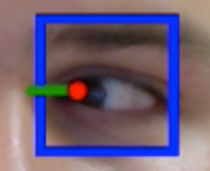
\includegraphics[width=1.3in]{figs/gazePrediction.pdf}

    \caption{Determining the Gaze Metric}

\end{figure}

 Since the gaze metric represents the pupil's displacement from the center, it
 can be represented as a 2D vector. In \textbf{Figure 2}, this vector is being
 drawn from the pupil center. This gives us a visual representation of the gaze
 direction. This metric is also used in calibration so that we can interpolate
 the position on the screen that user is looking.

\subsection{Calibration}

Calibration in an eye tracking system is necessary to ensure that the predicted
point of gaze resembles the expected point of gaze. The calibration creates a
mapping from what the eye tracker determines the gaze metric is to a point on
the screen. For visible light based eye tracking using commodity eye trackers,
neural network \cite{holland2012eye} and linear based calibration techniques
have been deployed. In our work, we use a linear based approach due to ease of
implementation and computing power restrictions imposed by doing the
computation inside the browser in real-time.

The linear approach works by placing sample points in the corners of the
viewing screen and asking the user to look at these points, one at a time.
Using the data gathered from the eye tracker and the knowledge of what point
the data corresponds to on the screen, we can construct a linear mapping from
the gaze metric onto the screen. We map the distance between the uncalibrated
point on the top left and  the uncalibrated point on the top right to the width
of the screen.  We also map the distance between the uncalibrated top left
point the uncalibrated bottom right point to the height of the screen. This
mapping determines parametric equations that be used to interpolate the gaze
point on the screen.

The system corresponds a box determined by the user's prompted gaze direction
to the box defined by the prompt locations, and determines a linear mapping
between the two boxes that is used to define screen coordinates from subsequent
gaze measurements. The application we created for calibration presents a point
in each corner of the screen, one at a time. The user then has 7 seconds to
look at the point before the next point is shown.

\subsection{Obtaining Video Data}

%\begin{figure}[ht]
%
%    \centering
%
%    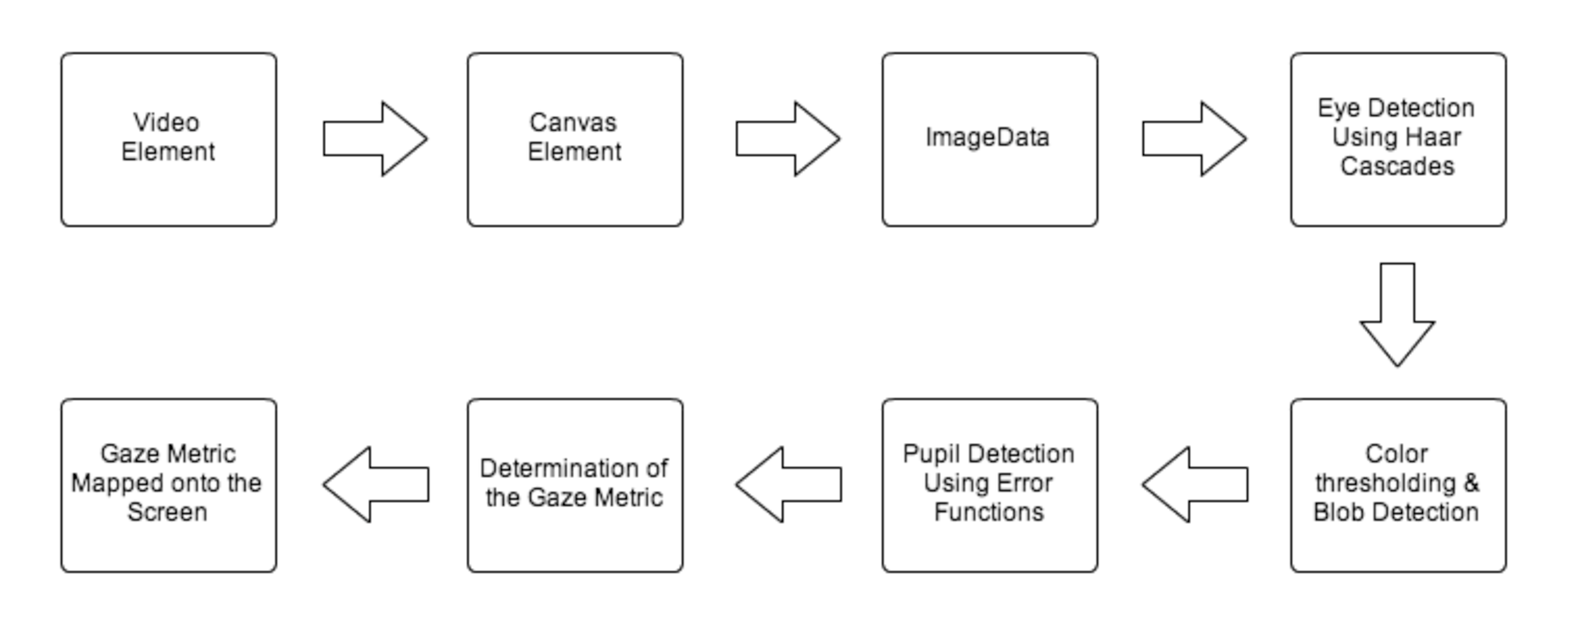
\includegraphics[width=3in, height=2in]{figs/Camgaze.pdf}
%    \caption{Structure of Camgaze.js Implementation}
%
%\end{figure}

Due to constraints imposed by JavaScript as a language while writing computer
vision applications, there are certain steps that need to be taken when
implementing the algorithms described above. Firstly, a video tag needs to be
already present in the HTML or created by the JavaScript application in order
for a video feed to be retrieved from the camera. Likewise, a canvas element
needs to be present in the HTML in order to retrieve the RGBA pixel values for
the video.  This is because the video element needs to be drawn onto the canvas
in order to retrieve the $\Acronym{ImageData}$ object for it. Once the
$\Acronym{ImageData}$ has been obtained, processing mentioned above can take
place.

\section{Methodology}

\subsection{Apparatus}

For the test we used an Apple MacBook Pro 13' laptop (mid-2013 model: Intel
Core i7 processor running on 2.9 GHz clock speed, 8 GB of RAM, 1280x800 screen
resolution).  It is equipped with a built-in FaceTime HD Camera, capable of
recording video with 720p resolution. The computer was running Apple OS X
(10.8.2) and Google Chrome web browser (build 30.0.1599.66) at the time of the
experiment. The screen of the laptop was $90^{\circ}$ with the base.

The room where the experiments were held was equipped with mildly-bright
flourescent lamps and had no natural light access. 

\subsection{Procedure}

A simple test was created to measure the precision of gaze prediction. At
first, linear calibration is performed in order to ensure that the gaze will be
projected on the screen correctly. During the calibration phase, users are
asked to look at the circles that appear on the screen. The calibration points
are sequentially shown at the corners of the screen, each for 7 seconds (as
mentioned in Section 3.3).  After the calibration phase, the precision test
begins.  A monochromatic circle appears on the screen in a random location, 20
pixels from each border, being displayed for 7 seconds.  This is repeated 10
times.  For the precision testing, the average gaze point is being recorded.
There was no indication of where the tracker predicted the gaze to the user in
order to limit the bias imposed by this information.

We then calculate the distance between the average gaze point and the center of
the associated test circle, and denote this as the error. The 10 error
measurements are then averaged to determine the accuracy and the standard
deviation is calculated to determine the uncertainty in measurement.

\section{Results}

\subsection{Accuracy}

We have conducted 5 tests. The result of these tests are shown \textbf{Table 1}
along with the results from Holland and Komogortsev's experiments.
\shortcite{holland2012eye}.  The distance accuracy refers to the average radius
around the test point that tracker predicted the gaze to be. These results are
comparable to those of Holland and Komogorstev which implemented gaze
prediction on a unmodified common tablet \shortcite{holland2012eye}. Since the
constraints that exists when programming on a tablet and programming in
JavaScript (JavaScript can run on a tablet through a web browser), the accuracy
in the results can be compared.  Their work performed with better accuracy by
0.7 inches during their first phase and by 0.6 inches in the second phase. The
key factor in this difference is the existence of a computer vision library in
Objective-C but not in JavaScript.  Increasing the performance of the
implemented computer vision algorithms will lead to better results.

In general, we believe that the received results provide a positive indication
of the viability of conducting eye tracking in a web-based environment. This
work concentrates on creating a proof of concept implementation of an
in-browser, client side gaze prediction application. The conducted tests were
meant to show the feasibility of the proposed concept. The results are
preliminary due to limited testing and we believe that further testing and a
usability study should be done to determine the absolute accuracy that is
possible to achieve using $\Name$.

\begin{table}\caption{Accuracy in Gaze Prediction (Phase 1 and 2 come from
Holland and Komogortsev)}  \centering \begin{tabular}{l|l|l} \textbf{Metric} &
\textbf{Value} (in) & \textbf{Uncertainty} (in) \\ \hline Phase 1
\shortcite{holland2012eye} & 1.4 & 0.2 \\ Phase 2 \shortcite{holland2012eye}&
1.5 & 0.1 \\ Distance & 2.1 & 0.1 \end{tabular} \end{table}

\subsection{Performance}

We have conducted 5 tests to measure the performance of $\Name$. The tests are
the same as the accuracy tests except that the calibration phase is not needed.
Our results are computed by obtaining the amount of usable frames from a
testing session and dividing it by the session length. The sampling rate was
17.5 FPS ($\pm$ 4.5).  This is a strong indication that our system is
sufficient to run on a vast range of different devices.

Our performance degrades under poor lighting conditions. Since the
implementation of the Haar detector in JavaScript currently does not support
tree-based cascades, different lighting conditions affect the amount of frames
that eyes were detected. We have found the best results when the user has
limited light projected directly on the face. The distance to the camera is
also an impeding factor on the performance. The user needs to be about 1 ft
from the webcam for the best results.

\section{Discussion}

\subsection{Privacy Concerns}

$\Name$ is intended to bring eye tracking to larger-scale deployment.  This
intensifies the need to address the privacy concerns some users might have. The
library we describe attempts to do this in several ways.

When the user accesses a web page that uses $\Name$, they are prompted a
notice that the website is attempting to use the video from their computer.
This is the default behaviour of both Chrome and Firefox and this behaviour can
not be overridden by any website. $\Name$ displays a notice that explains how
this data will be used.  Thus, we prevent capturing the data from an unaware
user.

As previously mentioned, $\Name$ is implemented in Javascript. Since the
majority of modern web browsers have an built-in Javascript interpreter, it is
possible to do the eye tracking on the client-side. This allows the proposed
solution to avoid sending and storing the user’s video stream to an external
server. In general, we believe that sensible measures have been taken to
mitigate the potential privacy impacts.

\subsection{Limitations}

Currently, Camgaze.js lacks any spatial awareness between the camera and the
user. In some cases, due to specific change in alignment of the user the result
from the eye tracker will be imprecise. Likewise, a change in head pose
potentially disrupts the precision of $\Name$ (e.g. if the user is looking at
the center of the screen but starts to tilt his / her head down, the gaze
metric will predict the user looking up due to the displacement from the center
of the eye to the pupil).

The lack of well trained Haar classifiers also limits the ability of this work.
The current classifiers available in JavaScript are not as highly trained and
thus do not detect the eyes as frequently in different lighting conditions.
This causes problems with $\Name$ because a gaze metric can not be determined
and a point on the screen is not mapped.

%While the eye tracking is unlike to begin, if the user is not initially
%properly aligned (e.g. the head is strongly tilted), it does not adjust to the
%variations of the head position that are possible in the real environment.

\section{Future Research \& Applications}

Preliminary experiments show that $\Name$ is working on a tablet computer
(Google Nexus 7 -- 2013 version, Chrome Beta 30.0.1599.81, V8 3.20.17.13
Javascript engine), which brings a potentiall to bring eye tracking to a
variety of hanheld devices. Further research could address the feasibility of
eye tracking on even smaller devices such as smartphones and “phablets” (phones
with a screen wider than 5’ inches).

We hope to make progress with porting one of the popular Computer Vision
libraries to Javascript, thus allowing to apply the latest developments in the
field to the task that $\Name$ tries to solve.

Additional research on the normalization of the video stream could be done.
Porting some of the algorithms to Javascript would be a novel task.

We believe that $\Name$ should be used in cases where the simplicity and
scalability of deployment overweights the need for perfect precision of point
of gaze prediction. Ability to open a webpage, click “ok” on a pop-up bar, and
start eye tracking opens up possibilities for use of eye tracking for various
new applications, which were previously “solvable” by eye tracking, but not
applied outside the controlled lab environment.

For example, Heitger et al. have shown that impaired eye movements in
post-concussion syndrome patients indicate trauma on the brain that surpasses
the influence of intellectual ability \cite{Heitger2009}. The use of current
generation eye tracking hardware / software combinations makes a deployable
solution for testing concussions based eye movements difficult. $\Name$ has the
ability to be used in these deployable senarios such as Emergency Rooms,
ambulances, and sports centers.

\section{Conclusion}

In this paper, we have described the design and implementation of a in-browser,
client side eye tracker written in JavaScript. We have also discussed the
privacy benefits, limitations, and impact such a system would have on current
eye tracking applications. Through our evaluation, we have found our
implementation to be accurate to a radius of 2.1 inches ($\pm$ 0.1) and the
sampling rate to be 17.5 FPS.

The performance of the proposed system is influenced by many mutable
limitations and therefore has the potential to impove. This work represents an
eye tracking system that will have neglible deployment costs and higher
accessibility. However there exists a price in accuracy that the authors feel
is worth the benefits.

This material is based upon work supported by the National Science Foundation
under Grant No. CNS- 1062743.

\bibliographystyle{acmsiggraph}
\bibliography{paper}

\end{document}
